\chapter{火箭发动机推进原理}
\thispagestyle{empty}
\section{概述}
\noindent \textbf{1. 火箭发动机工作过程与能量转化}
{
	\begin{center}
		\begin{tikzpicture}[node distance=1.2cm]
			%定义流程图具体形状
			\node(O) [minimum height=0cm,draw, xshift = -9cm,,inner sep=8pt] {燃烧室};
			\node (B) [minimum height=0cm,draw, xshift = -4.25cm,node distance=3.5cm, inner sep=8pt] {喷管};
			\node (C) [minimum height=0cm,draw, xshift = 0cm,node distance=2cm, inner sep=8pt] {推力传递系统};
			
			%连接具体形状
			\draw[arrows={-Stealth}](-12cm,0cm) -- (O)  node[midway,above=0cm]{推进剂} node[midway, below = 0cm]{化学能};
			\draw[arrows={-Stealth}](O) -- (B) node[midway, above = 0cm]{高温高压燃气} node[midway, below = 0cm]{热能};
			\draw[arrows={-Stealth}](B) -- (C) node[midway, above = 0cm]{高速燃气} node[midway, below = 0cm]{动能};
			\draw[arrows={-Stealth}](C) -- +(3.4cm,0) node[midway,above=0cm]{飞行器} node[midway, below = 0cm]{动能};
		\end{tikzpicture}
		\captionof{figure}{火箭发动机工作过程与能量转化}
		\label{火箭工作过程与能量转化}
	\end{center}
}
\vspace*{-0.5em}
火箭发动机的工作过程和能量转化如图\ref{火箭工作过程与能量转化}所示,实际的误差如表\ref*{火箭实际误差}所示。

\begin{table}[!htb]
	\centering
	\setlength{\tabcolsep}{10mm}{
	\begin{tabular}{|c|c|c|c|}
		\hline
		主要过程 & 分析方法 & 实际过程效率 & 产生原因 \\
		\hline
		燃烧放热 & $Q = \dot{m} \Delta t$ & 燃烧不完全 & 液滴,不均匀等\\
		\hline
		燃气加热 & $\Delta T = UI\dot{m}c_\gamma$ & 热损失 & 壁面传热等\\
		\hline
		膨胀加速 & $\Delta E_k  = \Delta H$ &不完全膨胀 & 分离、摩擦等\\
		\hline
		反作用推进 & $F = \dot{m}I_J$ & 分离,非对称等 & \\
		\hline
	\end{tabular}
	}
	\caption{火箭发动机的实际过程与主要误差}
	\label{火箭实际误差}
\end{table}

\noindent 在分析时,做出以下假设以简化模型\vspace*{-0.5em}
\begin{itemize}
	\item 燃烧室内:完全燃烧,化学能全部转化为热能;\vspace*{-0.5em}
	\item 燃烧室内:忽略热损失,热能全部用于燃气升温;\vspace*{-0.5em}
	\item 喷管内:燃气绝热等熵流动,热能转化为动能。
\end{itemize}
\vspace*{-0.5em}

\section{推进系统的推力}
\subsection{牛顿三大定律}
\vspace*{-1em}
\theorem[牛顿三大定律]
{
	第一运动定律
	\begin{equation}
		\sum \bm{F}_i = \dfrac{\d \bm{v}}{\d t} = 0
	\end{equation}
	\hspace*{1.8em} 第二运动定律
	\begin{equation}
		\bm{F} = \dfrac{\d \bm{p}}{\d t} \qquad \bm{F} = \dfrac{\d m}{\d t}\bm{v} + m \dfrac{\d \bm{v}}{\d t}
	\end{equation}
	\hspace*{1.8em} 第三运动定律
	\begin{equation}
		\bm{F}_{12} = \bm{F}_{21}
	\end{equation}
}

其中,$\bm{F}$为力,$\bm{v}$为速度,$m$为质量,$t$为时间,$\bm{p} = m \bm{v}$为动量。
\vspace*{1em}

\subsection{推力公式}
\noindent \textbf{1. 假设条件(理想情况)}\vspace*{-0.5em}
\begin{enumerate}[\hspace*{1.5em} (1) ]
	\item 一维定常流动;\vspace*{-0.5em}
	\item 外界大气压均匀;\vspace*{-0.5em}
	\item 忽略推进剂入口造成的动量。
\end{enumerate}
\vspace*{1em}

\noindent \textbf{2. 推力公式的推导}
\begin{figure}[!htb]
	\centering
	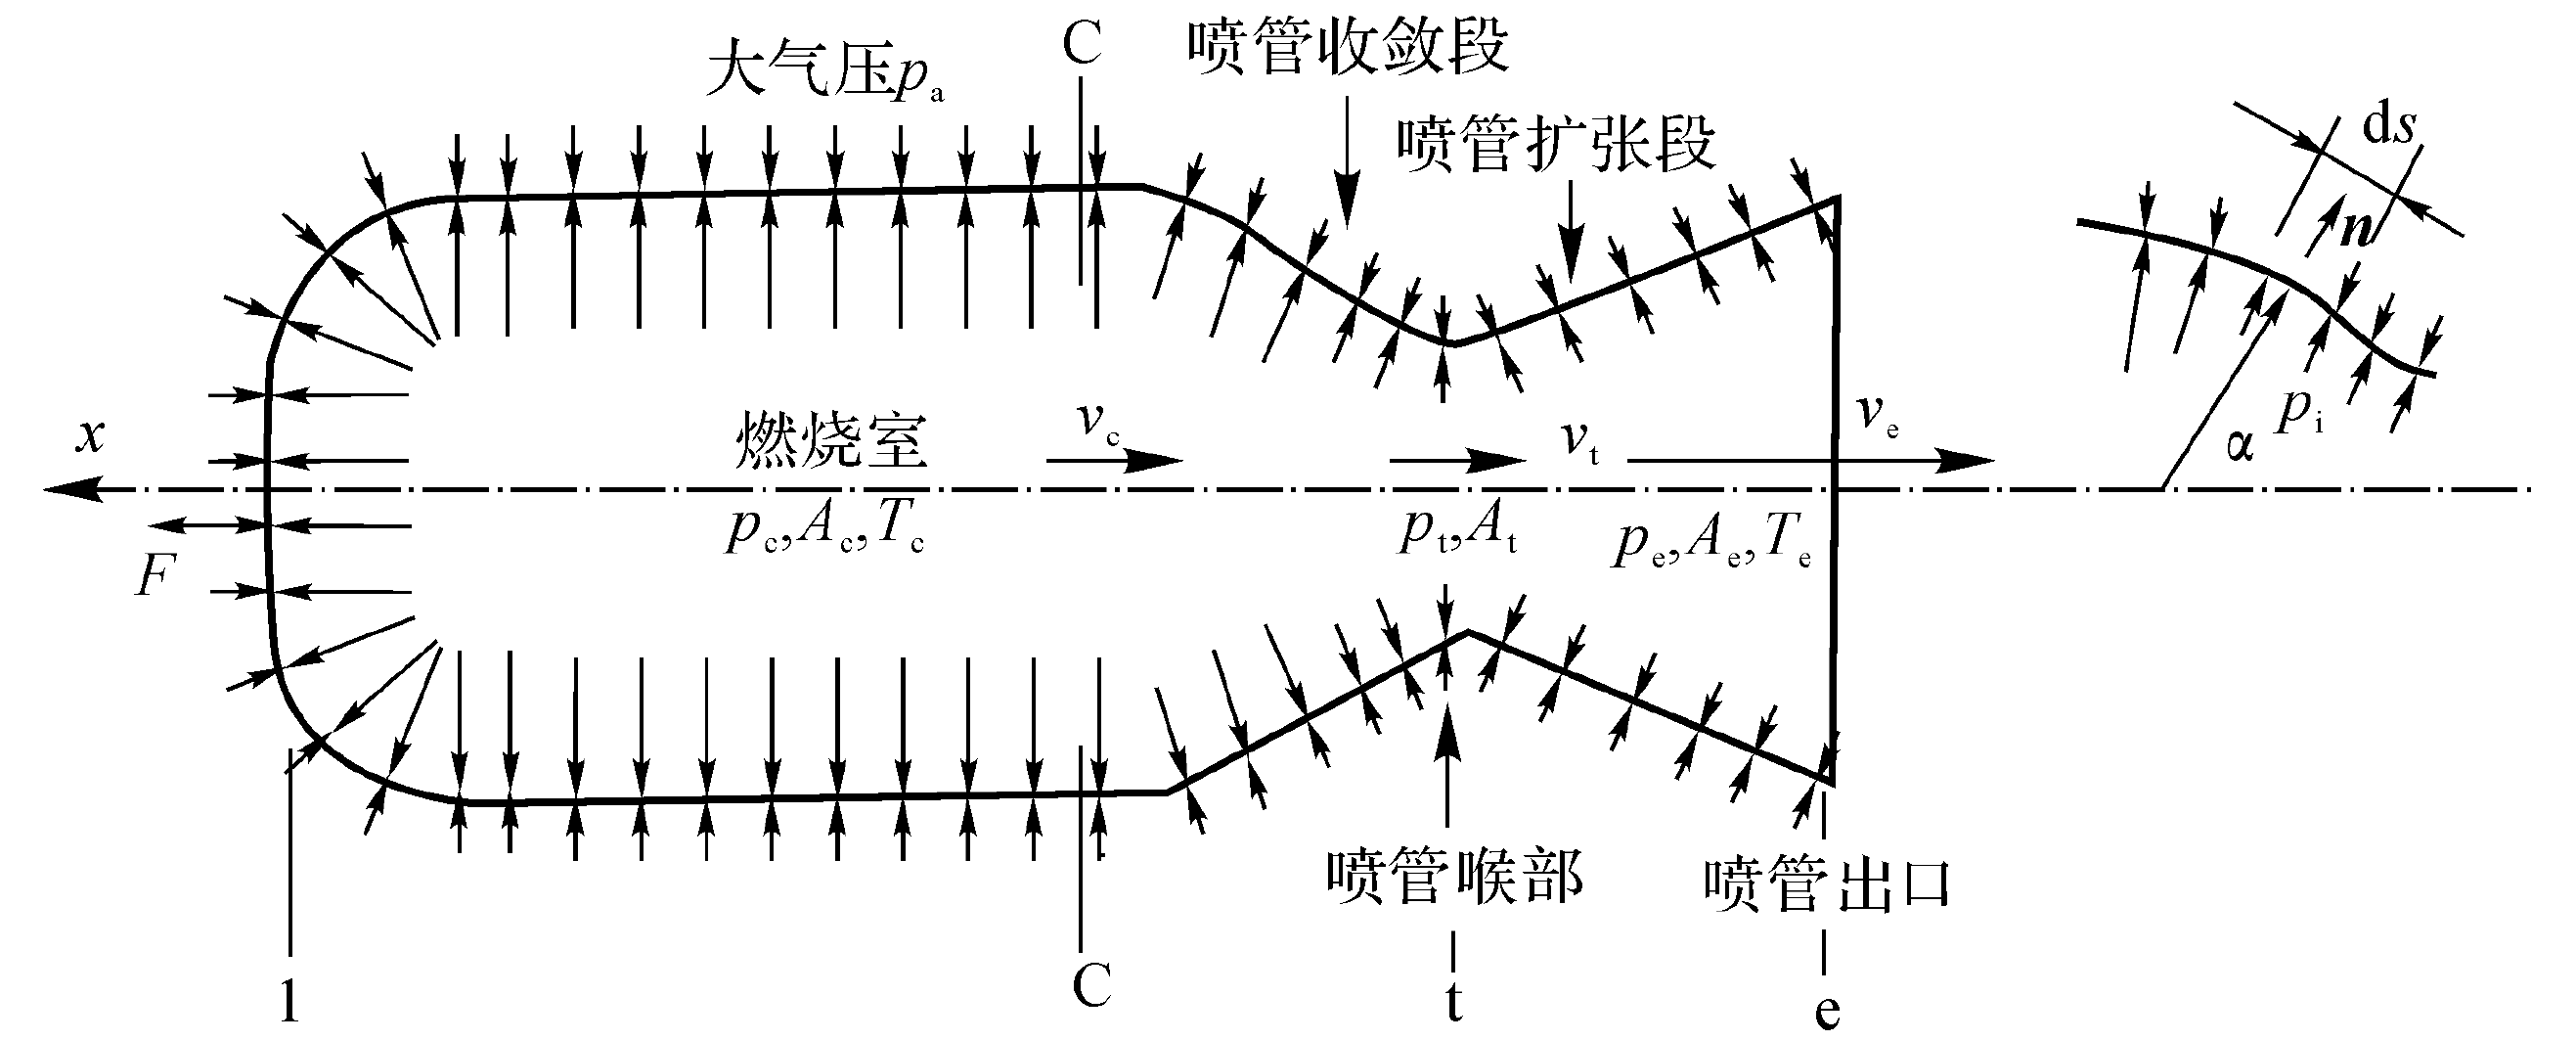
\includegraphics[width=0.8\linewidth]{pic/推力推导.png}
	\vspace*{-1em}
	\caption{火箭喷射示意图}
	\label{推力推导}
\end{figure}

如图\ref{推力推导}所示,火箭发动机在工作时不仅在内表面会受到燃气压强的作用,其外表面还会受到环境气压的作用,即
\begin{equation}
	\bm{F} = \bm{F}_{\text{in}} + \bm{F}_{\text{out}}
\end{equation}

取$x$方向为正方向,由于火箭是沿轴向对称的,垂直于轴线方向的力相互抵消,则只需考虑喷管的出口部分,由气体受到喷管出口向前的力(和速度方向相反),设$\bm{F}_{\text{in}}$方向为$x$轴正向,则由动量定理
\begin{equation}
		-\bm{F}_{\text{in}} - p_{\text{e}} \bm{n} A_{\text{e}} = m (\bm{u}_{\text{e}} - \bm{u}_{\text{in}})
\end{equation}
即
\begin{equation}
	\bm{F}_{\text{in}} = - m (\bm{u}_{\text{e}} - \bm{u}_{\text{in}}) - p_\e \bm{n} A_\e
\end{equation}
由气压外力与$x$轴正向方向一致,则
\begin{equation}
	\bm{F}_{\text{out}} = p_{\e}
\end{equation}
\vspace*{1em}

\noindent \textbf{3. 推力公式}

\theorem[推力公式]
{
	\quad \vspace*{-1em}
	\begin{equation}
		F = \mathop{\underbrace{\dot{m}u_\e}}_{\scriptsize \mbox{\blue[动量推力]}} + \,\,\, \mathop{\underbrace{(p_\e - p_\a)A_\e}}_{\scriptsize \mbox{\blue[压力推力]}}
	\end{equation}
	其中,\vspace*{-0.5em}
	{
		\begin{enumerate}[\hspace*{1.5em}]
			\item $\bm{F}$ \quad 推力,N \vspace*{-0.5em}
			\item $\dot{m}$ \quad 流量,kg/s \vspace*{-0.5em}
			\item $\bm{u}_\e$ \quad 火箭喷气出口速度, m/s \vspace*{-0.5em}
			\item $\bm{p}_\e$ \quad 火箭喷气出口压强,kPa \vspace*{-0.5em}
			\item $\bm{p}_\a$ \quad 当前高度的大气压强,kPa \vspace*{-0.5em}
			\item $A_\e$ \quad 火箭喷气出口的截面积,$\text{m}^2$ 
		\end{enumerate}
	}
}
\vspace*{1em}

\noindent \textbf{4. 推力公式的讨论}

(1) \hspace*{0.5em}$\dot{m}u_\e$为\dy[动量推力]{DLTL},占推力总值的90\%以上,$(p_\e - p_\a)A_\a$为\dy[压力推力]{YLTL}。

(2) \hspace*{0.5em}进入推力室燃料有初始速度?固体发动机和液体发动机。

(3) \hspace*{0.5em}火箭发动机的推力与飞行器的飞行速度无关,与高度(大气压强)相关。

(4) \hspace*{0.5em}实际飞行中,有外阻力? \quad \blue[有]

(5) \hspace*{0.5em}排气速度不均匀?非沿轴向?\quad 

(6) \hspace*{0.5em}是杏需要假设:完全气体假设?绝热等熵?无热损失和摩擦损失?\quad \blue[不需要]

\vspace*{1em}

\noindent \textbf{5. 推力相关概念}

\defination[特征推力]
{
	\dy[特征推力]{TZTL}(\dy[额定推力]{EDDL}、\dy[发动机设计状态推力]{FDJSJZTTL}):当$p_\e = p_\a$时的发动机推力。对应的高度为火箭发动机的设计高度。即$F^0 = \dot{m}u_\e$
}

\defination[真空推力]
{
	发动机在真空环境下工作时的推力,$P_\a = 0$,即$F_\text{V} = \dot{m}u_\e + P_\e A_\e$
}

\defination[地面推力(海平面推力)]
{
	\quad \vspace*{-1em}
	\begin{equation}
		F_0 = \dot{m}u_\e + A_\e (p_\e - p_{\a 0})
	\end{equation}
	 其中,$p_{\a 0}$为地面的大气压强。
}

\section{喷气速度与流量特性}
\subsection{喷气速度}

\noindent \textbf{1. 基本假设}

(1) \hspace*{0.5em}燃烧室内的燃气参数$T,P_\text{c}, \rho$处处相等,忽略燃烧室速度。

(2) \hspace*{0.5em}喷管中的流动是一维定常、等熵流动,且忽略燃气对喷管壁的传热和摩擦。

(3) \hspace*{0.5em}燃气是定压比热为常数的理想气体(量热完全气体)。

(4) \hspace*{0.5em}燃烧室内化学平衡,喷管内组分不变(冻结流)。
\vspace*{1em}

\noindent \textbf{2. 公式推导}

由假设可得燃气流动的能量守恒方程
\begin{equation}
	H + \dfrac{u^2}{2} = H_0
\end{equation}

在截面处,有
\begin{align*}
	&H_\c + \dfrac{u_\c^2}{2} = H_\e + \dfrac{u_\e^2}{2}\\
	\Rightarrow \quad& H_0 = H_\e + \dfrac{u_\e^2}{2}\\
	\Rightarrow \quad& u_\e = \sqrt{2(H_0 - H_\e)}
\end{align*}

将$H_\e = c_pT_\e, \quad H_0 =c_p T_\f$代入,得
\begin{equation}
	u_\e = \sqrt{2c_p(T_\f - T_\e)} = \sqrt{2c_p T_\f \left(1 - \dfrac{T_\e}{T_\f}\right)}
\end{equation}
对于绝热等熵流动,有
\begin{equation*}
	\dfrac{T_\e}{T_\f} = \left(\dfrac{p_\e}{p_\c}\right)^{\textstyle \frac{k-1}{k}}, \qquad c_p = \dfrac{k}{k-1}\dfrac{R_0}{MW}
\end{equation*}
则可以得到喷气速度方程。

\theorem[喷气速度方程]
{
	\vspace*{-1em}
	\begin{equation}
		u_e = \sqrt{\dfrac{2k}{k-1} \dfrac{R_0}{MW}T_\f \left[1 - \left( \dfrac{p_\e}{p_\c} \right)^{\textstyle \frac{k-1}{k}}\right]}
	\end{equation}
	其中,\vspace*{-0.5em}
	{
		\begin{enumerate}[\hspace*{1.5em}]
			\item $R_0$ \quad 通用气体常数,N \vspace*{-0.5em}
			\item $M$ \quad 燃气平均相对分子质量,g / mol \vspace*{-0.5em}
			\item $k$ \quad 比热比 \vspace*{-0.5em}
			\item $T_\f$ \quad 推进剂绝热燃烧温度,K
		\end{enumerate}
	}
}

\noindent \textbf{2. $u_\e$的影响因素}
\begin{enumerate}[\hspace*{1em}(1) \hspace*{0.5em}]
	\item $T_\f$\quad $t_\f \uparrow$,可转换成动能的热能增加$\rightarrow u_\e \uparrow$
	\item $MW$ \quad $MW \downarrow \, \rightarrow \, u_\e \uparrow$
	\item $k$ \quad $k \uparrow \, \rightarrow\, \sqrt{\dfrac{2k}{k-1}}\, \bigg \downarrow$而$\displaystyle \left[1 - \left(\dfrac{p_\e}{p_\c}\right)^{\textstyle \frac{k-1}{k}}\right] \Bigg \uparrow\, \, \rightarrow$综合考虑,$u_\e$随$k$的增大而略有减小
	\item $\dfrac{p_\e}{p_\c}$ \quad 在$MW,k,T_\f$一定的情况下,$u_\e$随$\dfrac{p_\e}{p_\c}$的减小而增大。其物理意义为燃气在喷管中的膨胀程度,膨胀压强比$\dfrac{p_\e}{p_\c}$越小,燃气膨胀得越充分,有更多的热能转换为动能,喷气速度越高。若$p_\e = 0$,则说明此时燃气的全部热能都转换为动能,喷气速度达到极限值,称为\dy[极限喷气速度]{JXPQSD}。
\end{enumerate}

	\defination[极限喷气速度]
	{
		\vspace*{-1em}
		\begin{equation}
			u_{\text{L}} = \sqrt{2h_\c} = \sqrt{\dfrac{2k}{k-1} R T_\f}
		\end{equation}
	}

\section{飞行器飞行性能指标及分析}

\subsection{飞行器加速度特性}
简化飞行过程,垂直升空的起飞加速度为
\begin{equation}
	a = \dfrac{F}{m_0} - g_0 \quad \Rightarrow \quad \dfrac{a}{g_0} = \dfrac{F}{mg_0} - 1
\end{equation}
\dy[起飞推重比]{QFTZB}定义为$\dfrac{F}{m_0g_0}$,大飞行器约为1.2$\, \sim \,$2.2,小导弹约为$50 \, \sim \, 100$.

\subsection{小结}
航天飞行器或火箭飞行器的主要性能参数:最大速度$V_{\max}$(单级火箭),速度增量$\Delta V$(多级火箭),有效载荷,最大射程,最大飞行高度等
\vspace*{0.5em}

\noindent \textbf{1. 性能最佳}
\begin{enumerate}[\hspace*{1.5em} (1)  ]
	\vspace*{-0.5em}
	\item 有效载荷确定时,缩短完成任务的时间\vspace*{-0.5em}
\end{enumerate}

\vspace*{0.5em}
\noindent \textbf{2. 改进推进系统性能提高飞行器性能途径}
\begin{enumerate}[\hspace*{1.5em} (1)  ]
	\vspace*{-0.5em}
	\item 有效出口速度或比冲:直接影响飞行性能。方法:高能推经剂,高室压及大膨胀比喷管(高空上面级)\vspace*{-0.5em}
	\item 质量数增大:对数影响效果。方法:减小结构质量,增大起飞质量,采用多级推进。\vspace*{-0.5em}
	\item 加大起飞推力,缩短动力飞行时间,减少重力损失\vspace*{-0.5em}
	\item 减小阻力\vspace*{-0.5em}
	\item 最优喷管设计\vspace*{-0.5em}
	\item 发射初速度\vspace*{-0.5em}
	\item 有效喷出速度接近飞行器主飞行段的飞行速度
\end{enumerate}

\vspace*{0.5em}
\noindent \textbf{3. 任务速度}

\defination[任务速度]
{
	\dy[任务速度]{RWSU}:
}


\section{本章总结}
\begin{figure}[!htb]
	\centering
	\begin{tikzpicture}
		\node (A) [draw, inner sep = 5pt]{发动机推力};
		\node (A1) [draw, inner sep = 5pt, right of = A, node distance = 9cm]{\makecell[c]{$F=\dot{m}u_e+A_e(P_e - P_a)$:牛顿定律;\\假设条件,推力公式的推导*及其应用}};
		\node (B) [draw, inner sep = 5pt, below of = A, node distance = 2.4cm]{排气速度};
		\node (B1) [draw, inner sep = 5pt, right of = B, node distance = 9cm]{$\displaystyle u_e = \sqrt{\dfrac{2k}{k-1}\rho_e  P_e \left[\left(\dfrac{P}{P_e}\right)^{\textstyle \frac{2}{k}} - \left(\dfrac{P}{P_e}\right)^{\textstyle \frac{k+1}{k}} \right]}$};
		\node (C) [draw, inner sep = 5pt, below of = B, node distance = 2.4cm]{流量特性};
		\node (C1) [draw, inner sep = 5pt, right of = C, node distance = 9cm]{$\dot{m} = A \sqrt{\dfrac{2k}{k-1} \rho_\e P_\e \left[ \left(\dfrac{P}{P_\text{e}}\right)^{\textstyle\frac{2}{k}} - \dfrac{P}{P_\e}^{\textstyle\frac{k+1}{k}}\right]} \Rightarrow \dot{m} = \dfrac{\Gamma}{\sqrt{RT_\f}}P_\e A_\text{t} = C_\text{D}P_\text{c}A_\text{t} = \dfrac{P_\text{c}A_\text{t}}{c^*}$};
		\node (D) [draw, inner sep = 5pt, below of = C, node distance = 2cm]{推力系数};
		\node (D1) [draw, inner sep = 5pt, right of = D, node distance = 9cm]{$F = C_\text{F}P_\text{c}A_\text{t}$,其物理意义及影响因素};
		\node (E) [draw, inner sep = 5pt, below of = D, node distance = 2.4cm]{总冲和比冲};
		\node (E1) [draw, inner sep = 5pt, right of = E, node distance = 9cm]{$\displaystyle I = \int_0^{t_a} F\, \d t, \quad I_s = \dfrac{I}{M_P} = \dfrac{\displaystyle \int_0^{t_a} F \, \d t }{\displaystyle\int_0^{t_a} \dot{m}\, \d t}$,其物理意义、相关概念及影响因素};
		\node (F) [draw, inner sep = 5pt, below of = E, node distance = 2.4cm]{\makecell[c]{推进剂的混合比\\当量比、余氧系数}};
		\node (F1) [draw, inner sep = 5pt, right of = F, node distance = 9cm]{组元确定情况下,氧化剂和燃料之间的比值,决定燃烧室温度。};
		\node (G) [draw, inner sep = 5pt, below of = F, node distance = 2cm]{飞行器运动};
		\node (G1) [draw, inner sep = 5pt, right of = G, node distance = 9cm]{$F = M\dfrac{\d V}{\d t}\quad \red[V_{\max} - V_0 = \ln \mu] \quad M_0 = M_P + M_e + M_s$};
		\node (H) [draw, inner sep = 5pt, below of = G, node distance = 2cm]{\makecell[c]{飞行器性能\\与发动机性能关系}};
		\node (H1) [draw, inner sep = 5pt, right of = H, node distance = 9cm]{$\displaystyle \Delta u_f = \sum_{i = 1}^{n} I_{s_i} \ln \mu_i$};
		
		\draw[arrows={-Stealth[scale=0.8]}] (A) -- (B);
		\draw[arrows={-Stealth[scale=0.8]}] (B) -- (C);
		\draw[arrows={-Stealth[scale=0.8]}] (C) -- (D);
		\draw[arrows={-Stealth[scale=0.8]}] (D) -- (E);
		\draw[arrows={-Stealth[scale=0.8]}] (E) -- (F);
		\draw[arrows={-Stealth[scale=0.8]}] (F) -- (G);
		\draw[arrows={-Stealth[scale=0.8]}] (G) -- (H);
		\draw (A) -- (A1);
		\draw (B) -- (B1);
		\draw (C) -- (C1);
		\draw (D) -- (D1);
		\draw (E) -- (E1);
		\draw (F) -- (F1);
		\draw (G) -- (G1);
		\draw (H) -- (H1);
	\end{tikzpicture}
	\caption{第1章总结图}
	\label{第1章总结图}
\end{figure}
































